% !TeX program = xelatex
% Options for packages loaded elsewhere
\PassOptionsToPackage{unicode}{hyperref}
\PassOptionsToPackage{hyphens}{url}
\documentclass[
]{article}
\usepackage{xcolor}
\usepackage{amsmath,amssymb}
\setcounter{secnumdepth}{-\maxdimen} % remove section numbering
\usepackage{iftex}
\ifPDFTeX
  \usepackage[T1]{fontenc}
  \usepackage[utf8]{inputenc}
  \usepackage{textcomp} % provide euro and other symbols
\else % if luatex or xetex
  \usepackage{unicode-math} % this also loads fontspec
  \defaultfontfeatures{Scale=MatchLowercase}
  \defaultfontfeatures[\rmfamily]{Ligatures=TeX,Scale=1}
\fi
\usepackage{lmodern}
\ifPDFTeX\else
  % xetex/luatex font selection
\fi
% Use upquote if available, for straight quotes in verbatim environments
\IfFileExists{upquote.sty}{\usepackage{upquote}}{}
\IfFileExists{microtype.sty}{% use microtype if available
  \usepackage[]{microtype}
  \UseMicrotypeSet[protrusion]{basicmath} % disable protrusion for tt fonts
}{}
\makeatletter
\@ifundefined{KOMAClassName}{% if non-KOMA class
  \IfFileExists{parskip.sty}{%
    \usepackage{parskip}
  }{% else
    \setlength{\parindent}{0pt}
    \setlength{\parskip}{6pt plus 2pt minus 1pt}}
}{% if KOMA class
  \KOMAoptions{parskip=half}}
\makeatother
\usepackage{graphicx}
\makeatletter
\newsavebox\pandoc@box
\newcommand*\pandocbounded[1]{% scales image to fit in text height/width
  \sbox\pandoc@box{#1}%
  \Gscale@div\@tempa{\textheight}{\dimexpr\ht\pandoc@box+\dp\pandoc@box\relax}%
  \Gscale@div\@tempb{\linewidth}{\wd\pandoc@box}%
  \ifdim\@tempb\p@<\@tempa\p@\let\@tempa\@tempb\fi% select the smaller of both
  \ifdim\@tempa\p@<\p@\scalebox{\@tempa}{\usebox\pandoc@box}%
  \else\usebox{\pandoc@box}%
  \fi%
}
% Set default figure placement to htbp
\def\fps@figure{htbp}
\makeatother
\ifLuaTeX
  \usepackage{luacolor}
  \usepackage[soul]{lua-ul}
\else
  \usepackage{soul}
\fi
\setlength{\emergencystretch}{3em} % prevent overfull lines
\providecommand{\tightlist}{%
  \setlength{\itemsep}{0pt}\setlength{\parskip}{0pt}}
\usepackage{bookmark}
\IfFileExists{xurl.sty}{\usepackage{xurl}}{} % add URL line breaks if available
\urlstyle{same}
% fallback for those not using the hyperref driver hyperxmp:
\makeatletter
\@ifundefined{xmpquote}{\newcommand{\xmpquote}[1]{#1}}{}
\makeatother
\hypersetup{
  hidelinks,
  pdfcreator={LaTeX via pandoc}}

\author{}
\date{}

\begin{document}

\textbf{Supplementary materials for}

\textbf{Non-extreme Rainfall and Tide Synchronization Caused
Catastrophic Typhoon Flooding in 1905 Shanghai}

Shuai Wang \textsuperscript{1}, Yilong Niu \textsuperscript{2}, Zhan
Tian \textsuperscript{3}, Laixiang Sun \textsuperscript{4}, Qinghua Ye
\textsuperscript{5}, Ralf Toumi \textsuperscript{6}, Guangtao Dong
\textsuperscript{7}, Md Musfike Meraz \textsuperscript{1}

\textsuperscript{1} Department of Geography and Spatial Sciences,
University of Delaware, DE, 19706, USA

\textsuperscript{2} yyyyyyyyyyy

\textsuperscript{3} School of Environmental Science and Engineering,
Southern University of Science and Technology, Shenzhen, 518055, China

\textsuperscript{4} Department of Geographical Sciences, University of
Maryland, College Park, MD, 20742, USA

\textsuperscript{5} Deltares, Delft, the Netherlands

\textsuperscript{6} Department of Physical, Imperial College London,
London, UK

\textsuperscript{7} Shanghai Climate Center, Shanghai Meteorological
Service, Shanghai, China

This file includes the supplementary materials as follows:

Supplementary Text 1

Supplementary Figure 1

Supplementary Movie 1

\ul{Supplementary Text 1}

\ul{1905 Typhoon intensity reconstruction}

Because direct measurements of minimum central pressure (\(P_{\min}\))
were unavailable for the 1905 typhoon, we estimated \(P_{\min}\) from
daily surface pressure recorded in Shanghai (\(P_{sh}\)) during the 1905
event, environmental pressure (\(P_{env}\)), the distance from Shanghai
to the cyclone center (\(R_{sh}\)), and the radius of maximum wind
(\(R_{\max}\)). To establish the relationship among \(P_{\min}\),
\(P_{sh}\), \(P_{env}\), \(R_{\max}\) and \(R_{sh}\), we utilized a
previously developed analytic tropical cyclone wind profile model---the
λ model, based on which, the pressure profile from TC center can be
written as (i.e., Equation 13 in ref. \textsuperscript{1}):

\[P_{env} - P = \kappa\frac{1 - e^{- \frac{R^{2}}{2\lambda^{2}}}}{\frac{R^{2}}{2\lambda^{2}}}\ \ \ \ ,\ \ \ \ \ \ \ \ \ \ \ \ (1)
\]

where P is the near-surface pressure measured at one location within the
TC system, λ can be written as \(\lambda = \frac{R_{\max}}{1.89}\),
which is a numerical solution of the λ model \textsuperscript{2}, and κ
can be regarded as a simultaneous constant that is controlled by the
outflow temperature and TC inner-core structure.

We replaced λ with \(\frac{R_{\max}}{1.89}\) and applied Equation (1) at
the location of Shanghai and TC center, which yields:

\[P_{env} - P_{sh} = \kappa\frac{1 - e^{- \frac{{R_{sh}}^{2}}{0.56{R_{\max}}^{2}}}}{\frac{{R_{sh}}^{2}}{0.56{R_{\max}}^{2}}}\ \ \ \ \ \ and\ \ \ \ \ \ \ \ \ \ \ \ \ \ \ \ \ \ \ \ \ \ \ \ \ \ \ \ \ \ \ \ \ \ \ \ \ \ \ \ \ \ \ (2)\]

\[P_{env} - P_{\min} = \kappa\ \ \ \ \ \ .\ \ \ \ \ \ \ \ \ \ \ \ \ \ \ \ \ \ \ \ \ \ \ \ \ \ \ \ \ \ \ \ \ \ \ \ \ \ \ \ \ \ \ \ \ \ \ \ \ \ \ \ \ \ \ \ \ \ \ \ (3)\]

By dividing Equation (2) with (3) we have

\[\frac{P_{env} - P_{sh}}{P_{env} - P_{\min}} = \frac{1 - e^{- \frac{{R_{sh}}^{2}}{0.56{R_{\max}}^{2}}}}{\frac{{R_{sh}}^{2}}{0.56{R_{\max}}^{2}}}\ \ \ \ \ \ .\ \ \ \ \ \ \ \ \ \ \ \ \ \ \ \ \ \ \ \ \ \ \ \ \ \ \ \ \ \ \ \ \ \ \ \ \ \ \ \ \ \ \ \ \ \ \ (4)
\]

We then employed two other empirical equations showing, respectively,
the wind-pressure relationship \textsuperscript{3} and operational
estimation of \(R_{\max}\) \textsuperscript{ref.4}, i.e.,

\[V_{\max} = 6.7\left( 1010 - P_{\min} \right)^{0.644}\ \ \ \ \ \ and\ \ \ \ \ \ \ \ \ \ \ \ \ \ \ \ \ \ \ \ \ \ \ \ \ \ \ \ \ \ \ \ \ \ \ \ \ \ (5)\]

\[R_{\max} = 66.785 - 0.09102V_{\max} + 1.0619(\phi - 25)\ \ \ \ \ \ ,\ \ \ \ \ \ \ \ \ \ \ \ \ \ \ \ \ \ \ \ \ \ \ \ \ \ \ \ \ \ \ \ (6)\]

where \(V_{\max}\) is the maximum wind speed, and \(\phi\) is the
latitude of TC center.

There are three unknowns in Equations (4)-(6), which are \(P_{\min}\),
\(V_{\max}\), and \(R_{\max}\). By plugging in the observations of
\(P_{sh}\), \(R_{sh}\), and \(P_{env}\) (with a value of 1010 hPa), we
empirically estimated the minimum central pressure of the 1905 Shanghai
Typhoon.

Figure S1 shows the estimated typhoon intensity along its track. We
noted that this approach may include considerable uncertainty for TC
intensity estimation. However, the main point of this study is to
evaluate the partial contributions of different hydrological events by
calculating the difference between the control and sensitivity
simulations. Since the same TC intensity estimation was used in all
simulations, this uncertainty can be partly mitigated. More importantly,
the hydrological simulations, as will be shown later, obtains
consistently water depth at key locations as recorded in the historical
documents, which further increase the confidence in this TC intensity
estimation approach.

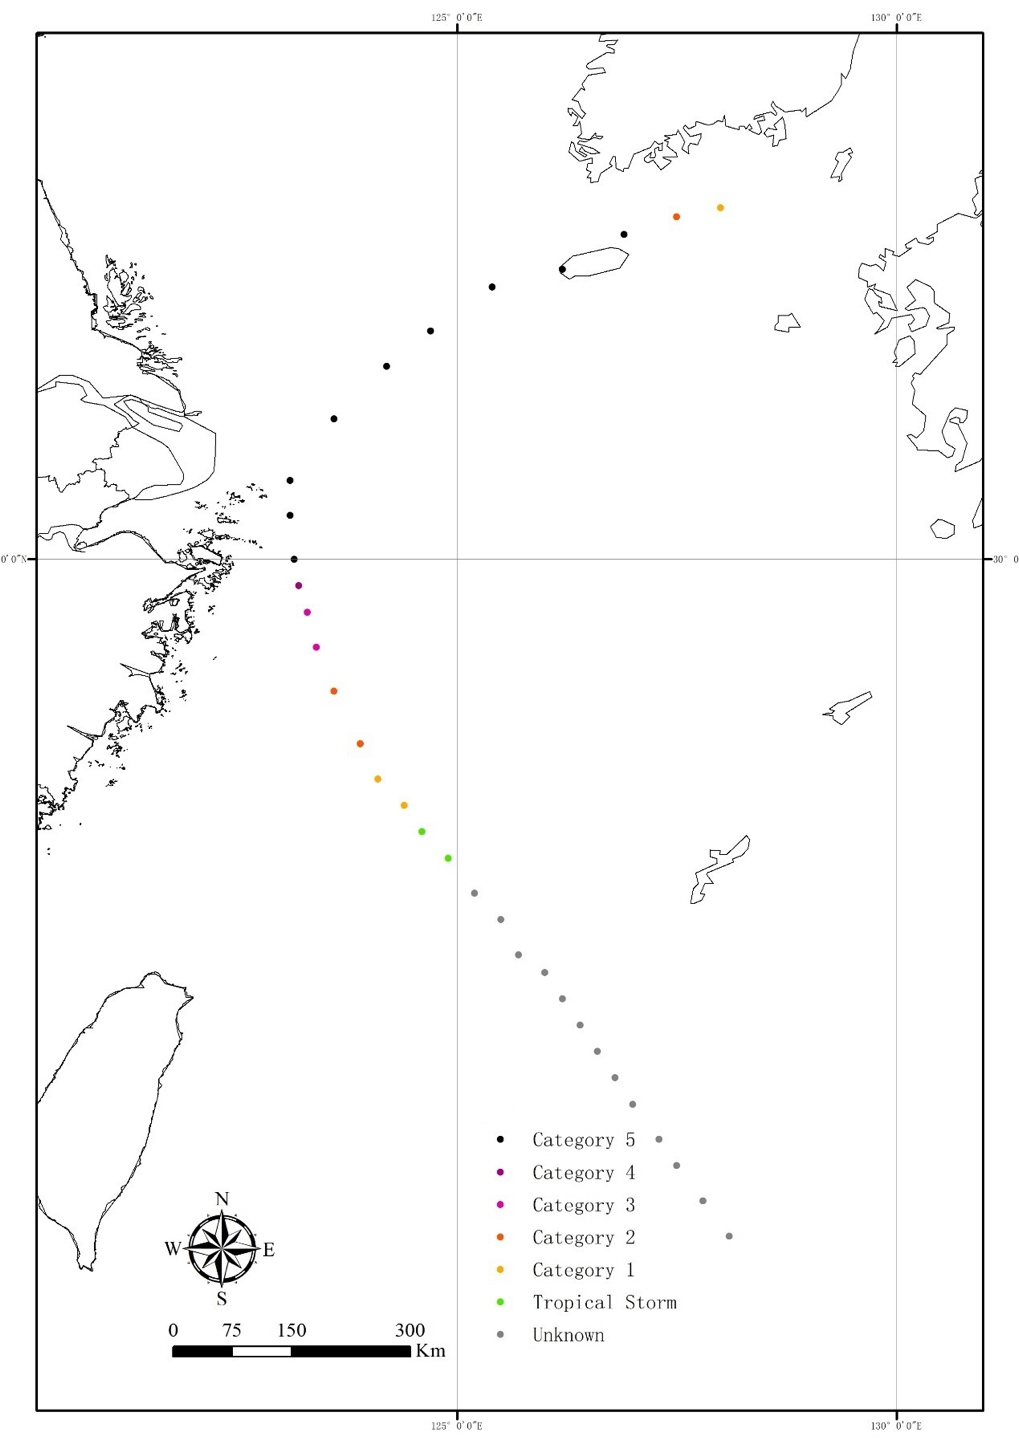
\includegraphics[width=4.62671in,height=6.54783in]{media_supp/media/image1.jpeg}

Supplementary Figure 1. Reconstructed 1905 Shanghai Typhoon intensity
following the storm track from the Atlas of the Tracks of 620 Typhoons,
1893--1918.

Reference

1. Wang, S., Toumi, R., Czaja, A. \& Kan, A. V. An analytic model of
tropical cyclone wind profiles. \emph{Quarterly Journal of the Royal
Meteorological Society} \textbf{141}, 3018--3029 (2015).

2. Wang, S. \& Toumi, R. On the relationship between hurricane cost and
the integrated wind profile. \emph{Environmental Research Letters}
\textbf{11}, 114005 (2016).

3. Atkinson, G. D. \& Holliday, C. R. Tropical Cyclone Minimum Sea Level
Pressure/Maximum Sustained Wind Relationship for the Western North
Pacific. \emph{Monthly Weather Review} \textbf{105}, 421--427 (1977).

4. Knaff, J. A. \& Zehr, R. M. Reexamination of Tropical Cyclone
Wind--Pressure Relationships. \emph{Weather and Forecasting}
\textbf{22}, 71--88 (2007).

\end{document}
